\chapter{Entwicklung}
Im folgenden Abschnitt sollen verschiedene Programmiersprachen, Programme und Code-Bib\-lio\-theken besprochen werden, welche bei der Verwirklichung dieses Projektes zum Einsatz kamen. 
Viele der erwähnten Programme und Bi\-bli\-o\-the\-ken sind Standardwerkzeuge der Entwicklung unter Linux und sind unter Open-Source-Lizenzen frei verfügbar. 

Um sowohl ein funktionierendes als auch bequem zu bedienendes Programm zu entwickeln, kamen auch mehrere Programmiersprachen zum Einsatz. Jede dieser Programmiersprachen hat ihre Stärken in 
einem bestimmten Bereich und es wurde versucht, jede Sprache nach ihrer individuellen Stärke einzusetzen. 

\section{C++}
\label{sec:cpp}
Als primäre Programmiersprache wurde C++ gewählt. Verschiedene Gründe sprachen für C++, unter anderem die an C angelehnte Syntax, aber
auch die gute Performance des generierten Maschinencodes im Vergleich zu Sprachen, welche üblicherweise in einer virtuellen Maschine laufen oder gar interpretiert werden. Zu 
all diesen Gründen kam noch hinzu, dass für C++ be\-reits ausgezeichnete Codebibliotheken zur Verfügung stehen, welche ein schnelles
und effizientes Arbeiten ermöglichen.

Bei C++ handelt es sich um eine im Jahr 1979 von Bjarne Stroustrup entwickelte Programmiersprache, welche anfangs als \textit{C mit Klassen}
ausgelegt wurde. Über mehrere Ent\-wick\-lungs\-schrit\-te entwickelte sich eine Sprache, dessen Wurzeln in der Sprache C immer noch zu erkennen sind, 
dessen Möglichkeiten jene von C aber bei weitem übersteigen. 

Wie C handelt es sich bei C++ um eine statisch-typisierte Programmiersprache, das heißt der Compiler kann schon während der Übersetzung die
syntaktisch korrekte Verwendung von Datentypen sicherstellen. Dadurch können solche Überprüfungen während der Ausführung des Programms
entfallen, was zu einer enormen Beschleunigung der Ausführung des Programms führt. Außerdem ermöglicht es dem Entwickler Fehler mit
inkorrekt verwendeten Datentypen einfacher zu erkennen, da eine Fehlermeldung des Übersetzers eine genaue Zeile angeben kann, in der 
der Fehler verursacht wird. 

Obwohl sich C++ wesentlich von C unterscheidet, ist es immer noch kompatibel mit C. Eine Stück C Code kann immer noch in C++ verwendet und
übersetzt werden. Dadurch können nicht nur Code-Bibliotheken aus dem C++-Umfeld verwendet werden, sondern auch ursprünglich für C gedachte
Bibliotheken eingebunden und verwendet werden. Da C immer noch eine der beliebtesten Programmiersprachen weltweit und vor allem \textbf{die}
Sprache für Systemprogrammierung und performante Software ist, bedeutet diese Mitnahme der Vorteile aus der C-Welt in die Welt von C++
einen großen Vorteil bei der Programmierung.

Des Weiteren wurde C++ möglichst plattformunabhängig designt. Während manche Funktionen, welche vom Betriebssystem bereit gestellt werden, 
natürlich nicht wirklich plat\-tform\-un\-ab\-hän\-gig sein können, wurde in C++ versucht, keine Funktionen oder Eigenschaften zu verwenden, welche
nur von einem bestimmten System ausgeführt werden können. Aus diesem Grund sind auch die meisten Code-Bibliotheken für C++ für die meisten
Plattformen erhältlich. 

Obwohl C++ wesentlich mehr Funktionen als C bietet, ist trotzdem noch die Anlehnung an C zu erkennen. Daher ist es auch nicht verwunderlich, dass C++-Programme meist nur geringfügig langsamer sind als 
vergleichbare C-Programme. In manchen Fällen ist C++ sogar schneller als C, da der Compiler andere, unter Umständen bessere, Optimierungen vornehmen kann. 

\subsection{STL}
\label{sec:stl}
Zusätzlich zu erwähnen ist die umfangreiche \textit{Standard Template Library (STL)}, welche es inzwischen sogar fast vollständig in den 
C++-Standard geschafft hat. Bei der STL handelt es sich um eine von den meisten Compilern bereitgestellte Code-Bibliothek für häufig 
verwendete Datenstrukturen und Hilfsroutinen, welche eine wesentliche Erleichterung für jeden C++-Programmierer darstellen. Unter anderem
in der STL enthaltene Datenstrukturen sind Listen, Stacks, aber auch Iteratoren für die meisten Datenstrukturen, sowie häufig verwendete Algorithmen
wie Quicksort oder Binarysearch. Hinzu kommen vereinheitlichte Ein- und Ausgabemöglichkeiten für verschiedenste Plattformen, sowie die 
Möglichkeit der parallelen Ausführung von Software mit Hilfe von Threads.

Die STL wurde inzwischen in den Sprachstandard von C++ aufgenommen, so dass jeder standardkonforme Compiler eine Implementierung der STL inkludiert. Mit der STL hebt sich C++ stark von C ab, für welches es keine solche allgemein einsetzbare Codebibliothek gibt. Der Preis für diese Einfachheit ist die Zeit, die ein einzelner Übersetzungsdurchgang benötigt. Da die STL stark auf die namensgebenden
\textit{Templates} setzt, welche es ermöglichen eine einzelne Datenstruktur für eine Vielzahl an Datentypen verfügbar zu machen, muss der Compiler diese \textit{Templates} zum Übersetzungszeitpunkt
auflösen, ein Vorgang, welcher einen stark negativen Einfluss auf die Übersetzungszeit hat.

\subsection{Einsatz}
Auf Grund der hohen Performance und der umfangreichen Code-Bibliotheken wurde für die Implementierung des Herzstückes dieser Arbeit C++ gewählt. Das bedeutet, dass alle Softwareteile, welche zur Lösung einer
einzelnen Probleminstanz gebraucht werden, als ein einzelnes Programm in C++-Quellcode vorliegt. Viele Hilfsroutinen, welche unter anderem dazu ge\-schrie\-ben wurden, neue Instanzen des PCP zu generieren, 
mehrere VNS-Instanzen gleichzeitig auszuführen und auch Auswertungen zu fertig berechneten Instanzen zu bieten, wurden hingegen in anderen Programmiersprachen geschrieben, welche zwar wesentlich langsamer
in ihrer Ausführung sind, dafür aber durch ihre Besonderheiten eine schnelle Programmentwicklung ermöglichen und auch einfach an neue Bedürfnisse angepasst werden können.

\section{Python}
\label{sec:python}
Neben der eigentlichen Applikation mit algorithmischem Kern entstanden im Laufe der Arbeit am Projekt zusätzliche Skripte, um repetitive Tätigkeiten zu beschleunigen. Unter anderem wurde Python zur massenhaften Ausführung des Algorithmus auf verschiedenen Testinstanzen und die anschließende Aufbereitung der Ergebnisse eingesetzt. Außerdem wurde diese Skriptsprache zur Konversion verschiedener Eingabeformate und zur Generierung von Eingabedaten verwendet.

Im Kontrast zur statisch typisierten Sprache C++ steht Python mit seinen dynamischen Eigenschaften, das heißt, dass Variablen grundsätzlich keinen statischen Typ aufweisen. Die so erhöhte Lesbarkeit wurde noch bewusst durch Whitespace-Konventionen und leichtgewichtige Syntax für Kontrollstrukturen und Schleifen erhöht. Außerdem ist die Python-Plattform (inklusive Interpreter) auf unixbasierten Systemen weit verbreitet, bei vielen Distributionen sogar Teil des Grundsystems. Hohe Popularität und gute Lesbarkeit als Design Pattern machen Python zu einer hervorragenden Skriptsprache, weshalb sie auch im Rahmen dieses Projektes in dieser Rolle Einsatz findet.

Während bei der Implementierung der Variablen Nachbarschaftssuche besonders die Performance zur Laufzeit berücksichtigt wurde, stand bei Skripten die Lesbarkeit und einfache Wartbartkeit im Vordergrund. Python passt auch hier ins Bild, da die Sprache üblicherweise interpretiert oder Just-In-Time übersetzt wird, was in der Regel eine höhere Laufzeit mit sich bringt. Dieser Nachteil relativiert sich dadurch, dass Scripts sowieso nicht als laufzeitkritische Teile des Projekts betrachtet werden.

\section{Make}
\label{sec:make}
Bei GNU make handelt es sich um ein Standardwerkzeug der Linux-Software-Entwicklung. Mit Hilfe von make kann die Übersetzung des Quellcodes in den Programmcode automatisiert werden. 
Dabei stellt make viele verschiedene Konfigurationsmöglichkeiten bereit. Unter anderem können verschiedene Compiler aber auch verschiedene Übersetzungsmodi eingestellt werden.
Um ein schnelleres Übersetzen zu ermöglichen werden außerdem nur jene Quellcode-Dateien neu übersetzt, welche sich seit dem letzten Mal verändert haben. 

In der Konfigurationsdatei für make, dem so genannten Makefile, können unter anderem mehrere \textit{Targets} angegeben werden, also quasi verschiedene Endprogramme oder verschiedene
Übersetzerkonfigurationen für das selbe Programm. Zu diesen \textit{Targets} werden dann Ab\-hängig\-keiten definiert welche bestimmen, in welcher Reihenfolge die einzelnen Quelltextdateien, aus denen das gesamte Projekt besteht, übersetzt werden 
müssen. Impliziert wird durch diese Abhängigkeitsdefinition auch, wann ein Programmteil neu übersetzt werden muss. Ist eine der Abhängigkeiten einer bestimmten Enddatei jünger als die 
Enddatei selber, muss diese neu übersetzt werden. Durch eine geschickte Aufteilung des Quellcodes auf mehrere Dateien kann so eine komplette Neuübersetzung in den meisten Fällen vermieden werden. 

Durch verschiedene Variablen, welche ebenfalls im Makefile spezifiziert sind, kann außerdem ohne großen Aufwand der Übersetzer, welcher die eigentliche Hauptaufgabe übernimmt, ausgetauscht werden.
Die für diese Arbeit verwendeten Compiler werden in Abschnitt~\ref{sec:compiler} besprochen. Vereinfacht wird dies durch die beinahe gleiche Befehlssyntax, die von beiden Compilern verwendet wird.
Hinzu kommt die Tatsache, dass die von den beiden Compilern erzeugten Dateiformate miteinander kompatibel sind, so dass auch bei uneinheitlicher Übersetzung mit immer wieder wechselnden Übersetzern
keine Fehler entstehen.

Außerdem hilfreich ist, dass make auch Skripte oder kleinere Kommandos automatisch aus\-füh\-ren kann. Häufig verwendet wird etwa die Routine zur Bereinigung des Programmverzeichnisses von bei der
Übersetzung entstandenen temporären Dateien, die später nicht mehr benötigt werden. Auch nützlich ist etwa die vollständige Entfernung jeder Spur einer Kompilierung, um eine gänzlich neue
Übersetzung einzuleiten. Weiters kann mit Hilfe von solchen Skripten das entstandene Programm nach der Übersetzung automatisch auf eine Testmaschine geschickt werden, um die korrekte Funktion
des Programmes zu verifizieren.

\section{Compiler}
\label{sec:compiler}
Der Compiler oder Übersetzer ist dafür verantwortlich, ein Programm von einer Quellsprache in eine Zielsprache zu übersetzen. Im Falle dieser Arbeit war die Quellsprache C++ und die
Zielsprache die Maschinensprache des Prozessors, also ein x86-Assembly. Übersetzer sind außerordentlich komplexe Stücke an Software, welche nicht einfach die Befehle eines Programmierers eins zu
eins übernehmen, sondern zusätzlich noch Optimierungen vornehmen, um eine beschleunigte Programmausführung zu ermöglichen. Da dieser Vorgang sehr zeitaufwendig sein kann ist es wichtig, Werkzeuge wie
das in Abschnitt~\ref{sec:make} besprochene make einzusetzen, um eine vollständige Neuübersetzung bei nur marginalen Änderungen im Quellcode zu verhindern. 

Da C++ eine besonders komplexe Sprache mit vielen verschiedenen, aufwendigen Funktionen und Sprachbesonderheiten ist, ist die Übersetzung eines C++-Quellcodes besonders aufwendig. Selbst kleinere
C++-Programme können schon mehrere Minuten zum vollständigen Übersetzen brauchen. Dies gilt insbesondere für Quellcode, welche die C++-Funktion der so genannten \textit{Templates} benützt. \textit{Templates}
erlauben es, neben anderen Dingen, eine allgemeine Datenstruktur für viele verschiedene Datentypen zu programmieren ohne eine konkrete Implementation für einen bestimmten Datentyp notwendig zu machen.
Da auch mehrere \textit{Templates} geschachtelt werden können und dies alles zum Zeitpunkt der Übersetzung expandiert werden muss, um schließlich übersetzt werden zu können, kann bei starker Verwendung
von solchen Funktionen die Geschwindigkeit der Übersetzung stark beeinträchtigt werden.

Um diese Probleme mit \textit{Templates} elegant zu umgehen, existiert das Konzept der \textit{Precompiled Headers}. Normalerweise werden Header-Dateien, welche allgemeine Deklarationen von Klassen, verwendeten Datentypen
und ähnliches enthalten, zum Übersetzungszeitpunkt in den C++-Quellcode, welcher übersetzt werden soll, komplett kopiert und diese Gesamteinheit als eine Über\-setzungs\-einheit angesehen. Dadurch muss, sollte
sich ein Teil der Definitionen innerhalb des C++-Codes ändern, auch die Definition neu übersetzt werden. Mit \textit{Precompiled Headers} wird dieses Problem gelöst, indem schon der Header als zu übersetzende und vom eigentlichen Quelltext abgetrennte Einheit angesehen wird. Der Header, welcher ja unter anderem auch die Deklarationen für \textit{Templates} enthält, muss nur noch
übersetzt werden, wenn sich in seinem eigenen Code etwas ändert. Dadurch können die eigentlichen Programmabschnitte, welche in normalen C++-Quelldateien zu finden sind, wesentlich schneller
compiliert werden ohne auf die Vorteile von \textit{Templates} zu verzichten.


\subsection{GCC}
GCC, die GNU Compiler Collection, ist eine Sammlung an Übersetzern, welche alle unter der Open-Source-Lizenz GPL veröffentlicht wurden. GCC wird häufig als der Standard-Compiler unter Linux angesehen
und erfreut sich immer noch großer Beliebtheit. Die Sammlung unterstützt viele verschiedene Sprachen, unter ihnen auch C++, sowie mehrere verschiedene Standards einzelner Sprachen. Auf Grund seiner
ausgiebigen Testung und Erprobung im all\-täg\-lich\-en Einsatz und nicht zuletzt seiner freien Verfügbarkeit bleibt GCC immer noch einer beliebtesten Compiler weltweit. Dabei ist die Sammlung verschiedener
Compiler vor allem im Umfeld der Softwareentwicklung für Linux beliebt, er kann aber auch für die Entwicklung unter Windows oder anderen Betriebssystemen eingesetzt werden.

Ein wichtiges Merkmal von \textit{g++}, dem C++-Compiler in der Sammlung der GCC, ist sein evolutionäres Wachstum seit seiner Entstehung. Da C++ mit den Jahren immer wieder lei\-cht angepasst und um Funktionen
erweitert wurde, musste sich auch GCC anpassen, um mit diesen Änderungen Schritt zu halten. Daher wurden im Laufe der Jahre immer wieder Teile von \textit{g++} neu geschrieben, umgebaut oder durch
neue Funktionen ergänzt. Daraus ergeben sich aber Konsequenzen, welche unter anderem die Code-Qualität negativ beeinträchtigen. Zwar Implementiert GCC auch den neuesten Standard von C++, allerdings
ist die Qualität der Implementierung sehr stark abhängig von dem Alter des entsprechenden Standards. Während ältere Standards bereits ausgiebig getestet wurden, ist bei neuen Standards eine korrekte 
Implementierung nicht immer gegeben. 

Auf Grund dieser gewachsenen Struktur von GCC ist der \textit{g++}-Compiler nicht der schnellste Vertreter seiner Art. Vor allem die Übersetzung von Headern nimmt mit der GCC mehr Zeit in Anspruch als
bei der Konkurrenz. Wie viele andere Compiler unterstützt auch \textit{g++} die Übersetzung von Header-Dateien in \textit{Precompiled Headers}. Dazu wird ein GCC-eigenes Format verwendet und \textit{g++} sucht bei einer
späteren Einbindung eines Headers in den Quellcode nach einer gleichnamigen Datei mit der Endung \enquote{.gch}. Die Verwendung von solchen \textit{Precompiled Headers} beschleunigt die Übersetzung ungemein, 
weil die Übersetzung des Headers selber einige Zeit in Anspruch nimmt. Die für diese Arbeit verwendeten \textit{Precompiled Headers} bewegten sich in der Größenordnung von knapp über 100 Megabyte, 
eine erstaunliche Datenmenge für eine einzige Übersetzungseinheit. Diese Datenmengen sind vor allem den \textit{Templates} geschuldet, welche während ihrer Expansion wesentlich an Speicherbedarf zunehmen.

\subsection{clang}
Bei clang handelt es sich um einen neuen Konkurrenten für GCC am Markt der Open-Source-Compiler. Wie bei GCC handelt es sich bei clang nicht um einen einzelnen Übersetzer für eine einzelne Programmiersprache,
sondern viel mehr um eine Sammlung an Übersetzern für vor allem mit C verwandten Sprachen wie C++ und Objective-C. Anders als GCC ist clang aber nicht über mehrere Jahrzehnte angewachsen, das Projekt
startete erst vor wenigen Jahren. Auch baut clang nicht von Grund auf auf einen neuen Compiler sondern benützt das Rahmenwerk der LLVM, der \textit{Low Level Virtual Machine}. LLVM ist ein Projekt, welches
mit dem Ziel gestartet wurde, Techniken des Just-in-Time-Übersetzens zu den Sprachen C und anderen Low-Level-Sprachen zu bringen. Dazu wird eine eindeutige Zwischensprache zwischen Quell- und Zielsprache
definiert, welche dann von LLVM optimiert werden kann. Diese Technik, welche ursprünglich zur Laufzeit eines Programmes zum Einsatz kommen sollte, wurde schließlich so adaptiert, um einen Compiler von
eben jener Zwischensprache zur Zielsprache zu bilden. 

Clang wurde nun mit dem Ziel geschaffen, einen sauber programmierten, standard-konformen Compiler für den produktiven Einsatz zu schaffen. Dazu wurde zunächst vor allem auf die Entwicklung eines C-Frontends
Wert gelegt. Als das C-Frontend einen arbeitsfähigen Zustand erreichte beschloss man, auch C++ als Quellsprache mit einzuschließen. Da C++ eine sehr umfangreiche Sprache mit vielen verschiedenen Spracheigenschaften 
ist, schreitet die C++-Implementierung wesentlich langsamer voran als jene des C-Zweiges. Inzwischen hat aber auch dieser Entwicklungszweig einen produktiven Zustand erreicht. 

Im Vergleich mit GCC bietet clang vor allem den Vorteil der Geschwindigkeit. Ein einzelner Übersetzerlauf dieser Arbeit ist um durchschnittlich 20\% schneller als mit GCC und die erzeugten Object-Dateien
sind um durchschnittlich 30\% kleiner. Dieser Vorteil ist wohl der neueren Programmierung ohne Mitnahme von Altlasten geschuldet. Der Preis für diesen Vorteil ist eine etwas langsamere Programmausführung
des fertig übersetzten Programmes, da unter anderem GCC einige Optimierungsmöglichkeiten nutzt, welche LLVM noch unbekannt sind. Im Allgemeinen sind die Unterschiede zwischen den beiden Compilern aber
vernachlässigbar gering.

\section{DDD}
DDD steht für Data Display Debugger und ist ein weiteres Werkzeug zur Softwareentwicklung von GNU\@. DDD stellt Werkzeuge zum Debuggen, also zur Fehlersuche in Software, zur Verfügung. Um produktiv eingesetzt
werden zu können muss eine spezielle Option während der Übersetzung mit GCC gesetzt werden, damit DDD einzelnen Programmschritten die richtigen Quellcodezeilen zuordnen kann. DDD ist eine sehr vielseitige
Anwendung mit graphischer Benutzeroberfläche, welche sehr intuitiv und einfach zu bedienen ist und trotzdem viele Optionen bietet. In Abbildung~\ref{img:ddd} wird beispielhaft die Verwendung von DDD im
Einsatz als Debugger dargestellt.

\begin{figure}
\centering
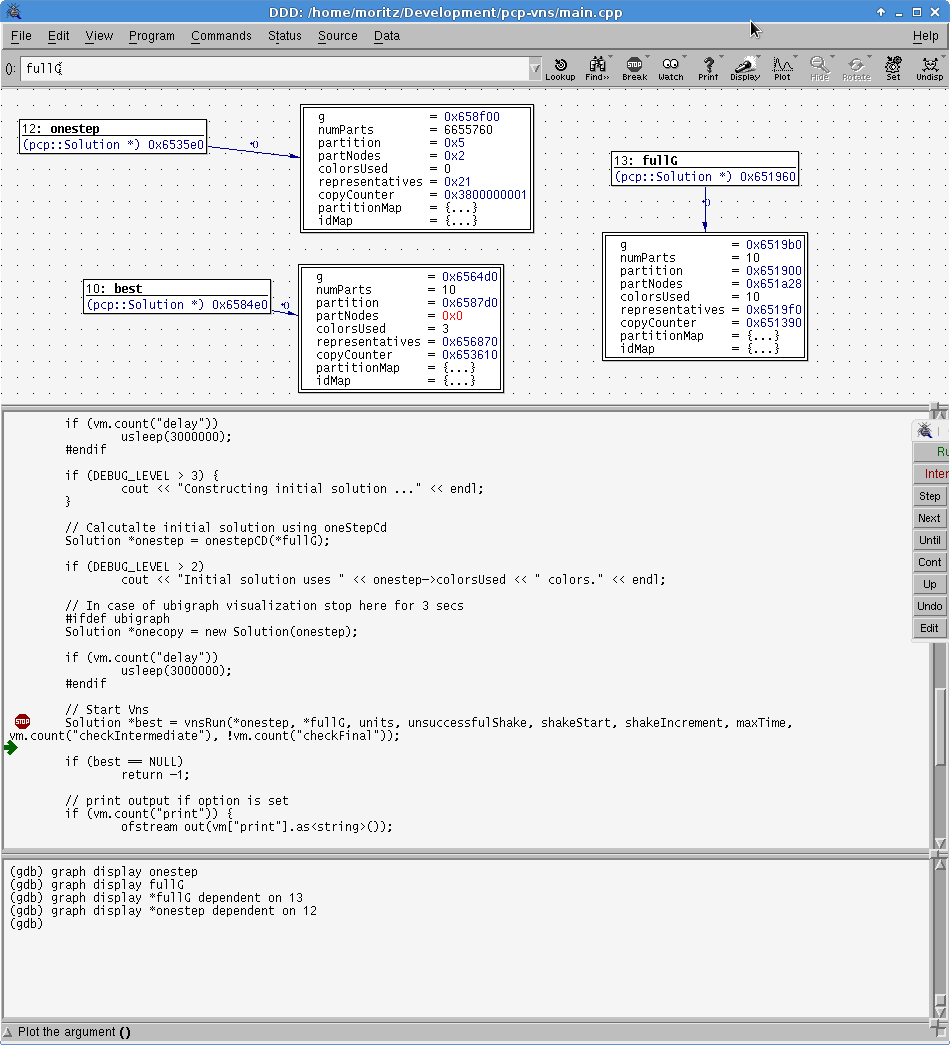
\includegraphics[width=0.8\textwidth]{img/ddd.png}
\caption[Beispielhafte Verwendung von DDD]{Beispiel eines Debuggingvorganges mit Hilfe des Werkzeuges DDD. Klar zu erkennen ist die Dreiteilung der Benutzeroberfläche.
Zuoberst befindet sich das Fenster für die Darstellung von Variablen, in der zur Zeit drei Referenzvariablen sowie ihr Inhalt dargestellt sind. Darunter folgt die Fläche für die Darstellung des Quellcodes.
Zu sehen ist ein Unterbrechnungspunkt (markiert durch das Stoppschild) sowie die derzeitige Position im Programmablauf (dargestellt durch den Pfeil). Am unteren Ende des Programmfensters ist die Befehlskonsole
zu finden, durch die einzelne Befehle, wie zum Beispiel das Starten und Anhalten des Programmes, gesteuert werden können.}
\label{img:ddd}
\end{figure}

Eines der wichtigesten Werkzeuge zur Fehlersuche innerhalb eines laufenden Programmes sind Unterbrechungspunkte, also eine bestimmte Stelle innerhalb des Quellcodes, an dem die Ausführung angehalten werden 
soll, um den genauen Zustand des Programmes zu untersuchen. DDD stellt sowohl normale Un\-ter\-brech\-ungs\-pun\-kte als auch spezielle Punkte, welche nur unter vom Benutzer definierten Bedingungen auslösen, bereit.
Sobald ein solcher Un\-ter\-brech\-ungs\-pun\-kt erreicht ist, kann DDD die Belegung sämtlicher Variablen anzeigen und vergleichen. Dies kann besonders nützlich sein, um ungeplantes Verhalten innerhalb des
Progamm\-ablaufes zu untersuchen und zu beheben. 

Außerdem bietet DDD die Möglichkeit, im Falle eines Programmabsturzes die auslösende Zeile des Quellcodes zu ermitteln und von dort aus auf die Ursachen des Absturzes zu schließen. Dies ist besonders
praktisch, da eine genaue Eingrenzung der Absturzursache ansonsten äußerst schwierig ist. Sollte ein Programm schadhaftes oder fehlerhaftes Verhalten an den Tag legen, zum Beispiel einen unberechtigten Speicherzugriff,
wird normalerweise das Programm sofort vom Betriebssystem beendet. DDD protokolliert aber jede aufgerufenen Zeile Code mit und kann daher genaue Auskunft geben, in welchem Programmabschnitt der
Fehler aufgetreten ist.

Ein weiteres praktisches Werkzeug von DDD ist die Möglichkeit, Pointer, welche auf vom Programm reservierte Speicherbereiche zeigen, genauenstens zu verfolgen. Durch eine übersichtliche graphische Darstellung
ist es einfach zu vergleichen, welche Pointer auf ein und den selben Speicherbereich zeigen, was unter Umständen gewollt sein kann oder aber auch einen fehlerhaften Programmablauf hervorruft.

\section{Boost}
\label{sec:boost}
Boost, oder auch Boost C++-Libraries, ist eine Codebibliothek welche versucht, Un\-zu\-läng\-lich\-keiten im Sprachstandard von C++ geschickt zu umgehen und Benutzern ein einfacheres Programmieren zu ermöglichen.
Boost besteht aus mehreren unabhängigen Unterbibliotheken, welche zum größten Teil unter der Boost Software Lizenz stehen, welche sowohl eine Open-Source als auch eine kommerzielle Nutzung zulässt. Alle
Unterbibliotheken sind portabel designt, um eine Nutzung auf allen Betriebssystemen mit C++-Compiler zu ermöglichen. 

Die Entwicklung von Boost begann im Jahr 2000, als Mitglieder des C++\--Standardisierungs\-komitees zusammentraten um Erweiterungen des C++-Standards auf einer breiteren öf\-fent\-li\-chen Plattform zu präsentieren.
Im Laufe der Entwicklung wurden immer wieder auch ehemals kommerzielle Produkte von Firmen in Boost eingegliedert, wie etwa die Graphikbibliothek GIL, welche ursprünglich von Adobe stammt, inzwischen
aber in den Boost-Stamm aufgenommen wurde.

Boost erweitert den Umfang an vorprogrammierten Datenstrukturen und auch Algorithmen und fügt bestehende Strukturen nahtlos ein. Dabei versucht Boost immer eine möglichst einfache und klar verständliche
Schnittstelle zu bieten, welche transparent mit Datenstrukturen etwa aus der STL umgeht, welche in Abschnitt~\ref{sec:stl} besprochen wurden. Von Boost geschaffene Datenstrukturen sind sehr ähnlich zu jenen
aus der STL zu verwenden und bieten wie jene auch einfache Möglichkeiten des Zugriffes auf Datenelemente über Iteratoren. 

Des Weiteren bietet Boost neue Möglichkeiten im Umgang mit Strings, also Zeichenketten, sowie weitere nützliche Hilfsfunktionen, welche von den meisten Programmen häufig gebraucht werden. Außerdem bietet
Boost Algorithmen und Datenstrukturen für mathematische Berechnungen, die über triviale Aufgaben wie addieren oder subtrahieren von einfachen Zahlen hinausgehen. So bietet Boost eine Unterbibliothek für 
Statistik und auch für Graphen, welche in dieser Arbeit zum Einsatz kam.

Außerdem wurden in dieser Arbeit viele Hilfsroutinen, welche von Boost bereitgestellt werden, verwendet: Auch kamen mehrere Datenstrukturen aus Boost-Unterbibliotheken zum Einsatz.

\subsection{graph}
\label{sec:boost:graph}
Da es sich bei dem PCP um ein Optimierungsproblem aus dem Umfeld der Graphentheorie handelt, ist natürlich eine Graphenstruktur innerhalb des Programmes unerlässlich. Boost bietet eine ganze Unterbibliothek, 
welche rein graphenbezogene Datenstrukturen und Algorithmen bereitstellt. Diese Graphenbibliothek ist gut getestet, vielseitig, stark anpassbar, schnell und einfach einzusetzen und war daher die ideale Wahl
für die Lösung des PCP\@.

Boost bietet zwei grundsätzlich unterschiedliche Implementierungen eines Graphen an. Bei der ersten Variante werden alle Kanten in einer Liste oder einer ähnlichen Datenstruktur gespeichert, bei
der zweiten Variante wird eine Matrix verwendet, um die Beziehungen zwischen zwei Knoten darzustellen. Während die zweite Variante für sehr dichte Graphen einige Vorteile bietet, ist die gesamte
Datenstruktur bei weitem nicht so flexibel wie die Variante mit einer Listenstruktur. In der von Boost verwendeten Implementierung dieser Adjazenzmatrix werden viele praktischen Funktionen, um einen
Graphen zu manipulieren, nicht unterstützt. So ist es zum Beispiel nicht möglich, einen Knoten nachträglich wieder zu entfernen. 

Daher fiel die Wahl auf eine Adjazenzliste, welche den Graphen für diese Arbeit bereitstellte. Auch hier gibt es mehrere verschiedene Konfigurationsmöglichkeiten, etwa die genaue Art der Speicherung von
Knoten und Kanten. Für die Speicherung der Knoten wurde ein Vektor gewählt, ein zusammenhängender Speicherbereich, welcher bei Bedarf vergößert oder verkleinert werden kann. Dies bietet mehrere Vorteile, etwa
einen direkten Zugriff auf einen Knoten über einen Index, welcher in Form einer einfachen ganzen Zahl leicht zu benützen war. Dies bedeutet, dass zu jedem Zeitpunkt direkt auf einen bestimmten Knoten zugegriffen
werden kann. Da die Anzahl der Knoten quasi immer konstant bleibt mit Ausnahme des erstmaligen Aufbaus des Problemgraphens und dem Errechnen der Initiallösung, werden die Nachteile einer vektorbasierten
Speicherung der Knoten bei weitem von den Vorteilen aufgewogen. 

Da im Rahmen der Variablen Nachbarschaftssuche mehrere Nachbarschaften immer wieder eine Veränderung der Adjazenzen vornehmen, fiel die Wahl der Datenstruktur für die Spei\-cher\-ung der Kanten zunächst auf eine
Liste. Zu jedem Knoten wird eine Liste der Nachbarknoten gespeichert, woraus dann die Kanten gebildet werden. Da das Löschen aus und das Einfügen in eine Liste in konstanter Laufzeit möglich ist, wurden
mit der Listenstruktur die besten Ergebnisse erwartet. Ausgiebige Tests ergaben jedoch, dass auch für die Speicherung der Kanten ein Vektor besser geeignet war. Da beim Löschen eines Knotens zumeist gleich alle adjazenten
Kanten gelöscht werden, reduzierte sich der Vorteil einer Listenstruktur und das Einfügen ist auch in einen Vektor in zumeist konstanter Zeit möglich. 

Eine weitere Konfigurationsmöglichkeit betrifft das Verhalten des Graphen beim Hinzufügen von Kanten. Es gibt gerichtete und ungerichtete Graphen, wobei gerichtete Graphen Kanten besitzen, welche quasi
als Einbahn fungieren, sie haben einen Anfangsknoten und einen Zielknoten und stellen nicht automatisch auch eine Verbindung vom Zielknoten zum Anfangsknoten her. Im Gegensatz dazu stehen die ungerichtete Graphen, bei denen
eine Kante automatisch eine Beziehung in beide Richtungen darstellt. Auf Grund der Eigenschaften des PCP fiel die Wahl auf einen ungerichteten Graphen, da kein Bedarf an gerichteten Kanten bestand.

Eine weitere von Boost bereitgestellte Funktion des Graphen ist die Speicherung von Eigenschaften im direkten Zusammenhang mit Kanten und Knoten. Da jeder Knoten im PCP zu einer Partition zugeteilt wird, kann
über diesen Mechanismus einfach und schnell von einem Knoten auf die Partition geschlossen werden. Diese Eigenschaften können außerdem dazu eingesetzt werden, den originalen Index eines Knotens zu speichern.
Da Boost bei der Entfernung eines Knotens automatisch den Index der nachfolgenden Knoten um eins dekrementiert, kann normalerweise nicht mehr auf den Index des Ursprungsknotens geschlossen werden. Durch
die Speicherung des Index in einer separat von Boost bereitgestellten, mitschrumpfenden Datenstruktur kann aber immernoch eindeutig auf den Originalknoten geschlossen werden. 

Eine einfache Möglichkeit der Ausgabe wird ebenfalls von Boost gestellt. Boost bietet eine einzelne Funktion, welche einen Boost-Graphen im Graphviz-Format ausgibt. Dadurch ergibt sich eine schnelle 
Möglichkeit, die Richtigkeit einer Lösung zu kontrollieren. Gerade bei frühen Versuchen der Nachbarschaftssuche wurde viel mit diesem Werkzeug gearbeitet, um die Ergebnisse zu verifizieren. 

\subsection{Hilfsroutinen}
Neben Graphen wurden auch einige von Boosts Hilfsfunktionen benutzt. Um bei der Lösung des PCP möglichst flexibel zu sein wurde eine Vielzahl an Variablen verwendet, um bestimmte Parameter der 
Nachbarschaftssuche einfacher ändern zu können. Dazu wurde angedacht, die Terminalparameter, als jene Parameter, welche beim Aufruf des Programmes über die Kommandozeile mitgegeben werden, zu verwenden. 
In einem ersten Versuch wurde ein einfaches Stringparsing betrieben, welches sich aber schnell als fehleranfällig herausstellte und zusätzlich noch zu unschönem Code führte. 

Genau für den Zweck der Programmargumente bietet Boost eine eigene Unterbibliothek, welche einem alle Aufgaben aus dem Bereich des Parsings übernimmt und dies außerdem noch in ei\-ner eleganten Art und Weise für
den Programmierer anbietet. Durch einen Bibliotheksaufruf können einfach neue Befehle angegeben werden und diesen Befehlen gleich ein bestimmter Datentyp zugeordnet werden. Es besteht aber nicht nur die 
Möglichkeit, einen bestimmten Datentypen zuzuordnen, sondern ein bestimmtes Argument gleich an eine Variable zu binden, sodass diese Variable automatisch von Boost gesetzt wird. Des Weiteren kann einem
Argument automatisch ein Standardwert zugewiesen werden welcher automatisch angenommen wird, sollte der Benutzer bei der Ausführung des Programmes dieses Argument nicht explizit angeben. 

Um eine möglichst genaue Zeitmessung für die statistische Auswertung der Ergebnisse zu erlangen, wurde die Zeitnehmungsbibliothek von Boost herangezogen. Boost stellt einfache Zeitnehmer bereit, um 
möglichst genaue Messergebnisse zu bekommen, welche im Millisekundenbereich liegen. Dies ist manchmal gar nicht so einfach, da etwa die normalen Zeitfunktionen nur auf Sekundenbasis arbeiten und eine 
genauere Zeitmessung zumeist über die abgelaufenen CPU-Zyklen erfolgt.

\section{Valgrind}
Valgrind ist, wie schon DDD, ein Werkzeug zur Fehlersuche in laufenden Programmen. Dabei spezialisiert sich Valgrind auf die korrekte Verwendung und Freigabe von Speicher. Mit Hilfe von Valgrind ist es
möglich, Speicherlecks aufzuspüren und zu schließen. Dafür überwacht Valgrind den Programmablauf und sämtliche Speicherzugriffe und gibt nach Beendigung des Programmes eine genaue Aufzählung an vergessenen Speicherbereichen und 
nicht sauber gelöschten Objekten (siehe Listing~\ref{lst:valgrind}) aus. 

Zum Zweck der Informationssammlung und zur besseren Darstellung der Ergebnisse sollte das eigene Programm wieder mit der Debug-Option des Compilers übersetzt werden. Dadurch kann Valgrind unter anderem die Zeile
anzeigen, in der das nicht gelöschte Objekt erzeugt wird und Informationen geben, ab wann ein Speicherbereich verloren gegangen ist. Außerdem ist zu beachten, dass durch diese Mitprotokollierung des 
Programmablaufes die Geschwindigkeit desselben stark beeinflusst wird. Daher ist es notwendig, bei Vorgängen, welche innerhalb des Programmes durch eine Ausführungszeit beschränkt werden, diese Zeit anzupassen, 
um eine korrekte und ausreichend lange Ausführung des Programmes zu gewährleisten. 

Wenn nun innerhalb des Programmes ein Stück Arbeitsspeicher reserviert wird, merkt sich Valgrind diesen Vorgang und protokolliert mit, wieviele Zeiger auf diesen Speicherbereich verweisen. Sollte nun irgendwann
kein einziger Zeiger mehr diesen Speicherbereich referenzieren, es wurden also quasi alle Variablen, die diese Information enthielten, verworfen oder überschrieben und der Speicherbereich wurde nicht wieder
freigegeben, so weiß Valgrind, dass dieser Speicher für das Programm verloren gegangen ist. Sollte sich dieser Vorgang wiederholen entsteht ein immer größer werdender Pool aus nicht freigegebenen Speicherbereichen, welche
nicht gelöscht wurden. Nachdem eine Low-Level-Programmiersprache wie C++ keine richtige automatisierte Speicherverwaltung wie andere Sprachen, z.~B.\ Java und C\# hat muss der Programmierer selbst für die 
Freigabe von reservierten Speicherbereichen sorgen. Daher ist es essentiell für gute Programmierung, alle erzeugten Objekte nach ihrer Verwendung wieder freizugeben, um so den exzessiven und sinnlosen Gebrauch von
Hauptspeicher zu verhindern.

\singlespacing
\lstinputlisting[language={},identifierstyle={},caption={Ausgabe von \texttt{valgrind -v --leak-check=full \ldots} bei vorhandenem Spei\-ch\-er\-leck.},label={lst:valgrind}]{valgrind.txt}
\setstretch{1.5}

Da die VNS in der Theorie eine endlose Schleife der Verbesserung darstellt und daher auch das Programm eine prinzipiell unbegrenzte Laufzeit besitzen sollte, ist die Frage der Spei\-cher\-ver\-walt\-ung essentiell.
Selbst kleinste Speicherlecks könnten, über einen langen Zeitraum betrachtet, zum Absturz des Programmes führen. Daher bietet Valgrind eine einfach zu nutzende und übersichtliche Möglichkeit, die Korrektheit
der Speicherverwaltung innerhalb des laufenden Programmes zu testen. 

\section{Graphviz}
Graphviz ist eine Sammlung an Software-Werkzeugen zur Visualisierung von Graphen. Jedes Werkzeug aus der Softwaresammlung liest dabei eine im sogenannten Graphviz-Format ge\-schriebene Datei ein und transformiert
sie auf bestimmte Art und Weise. Die Funktionen umfassen von der Entfernung von doppelten Kanten bis zur visuellen Ausgabe in Form einer PDF oder PostScript-Datei viele nützliche Bearbeitungsmethoden für 
Graphen. 

Da die im Abschnitt~\ref{sec:boost:graph} besprochene Implementation eines Graphen-Datentypes durch die Boost-Bibliothek eine automatische Ausgabe eines Graphen in das Graphviz-Dateiformat er\-möglicht, war 
eine Verwendung dieser Werkzeuge sehr naheliegend. Durch die vielen verschiedenen Programme, welche von Graphviz bereitgestellt werden, war es ein Leichtes, eine einfache Möglichkeit der visuellen Kontrolle
der Arbeitsergebnisse zu implementieren. Im Gegensatz zur im Abschnitt~\ref{sec:ubigraph} eingesetzten Echtzeitdarstellung der Vorgänge während des Ablaufes des Programmes wurde die Werkzeugsammlung dazu eingesetzt,
die Eingabe mit der Ausgabe zu vergleichen und zu verifizieren, dass eventuelle Fehler in der internen Prüfungsroutine des Programmes nicht dazu führten, dass falsche Lösungen plötzlich als zulässig angesehen würden. Konkret trägt die bildliche Darstellung der Instanz (siehe Abbildung~\ref{fig:graphviz:pre}) dazu bei, eine bessere Vorstellung des Konfliktgraphen zu gewinnen, um die Schritte zur Lösung (Abbildung~\ref{fig:graphviz:post}) lei\-ch\-ter nachvollziehen zu können.

\begin{figure}
	\centering
	\begin{subfigure}[t]{0.45\textwidth}
		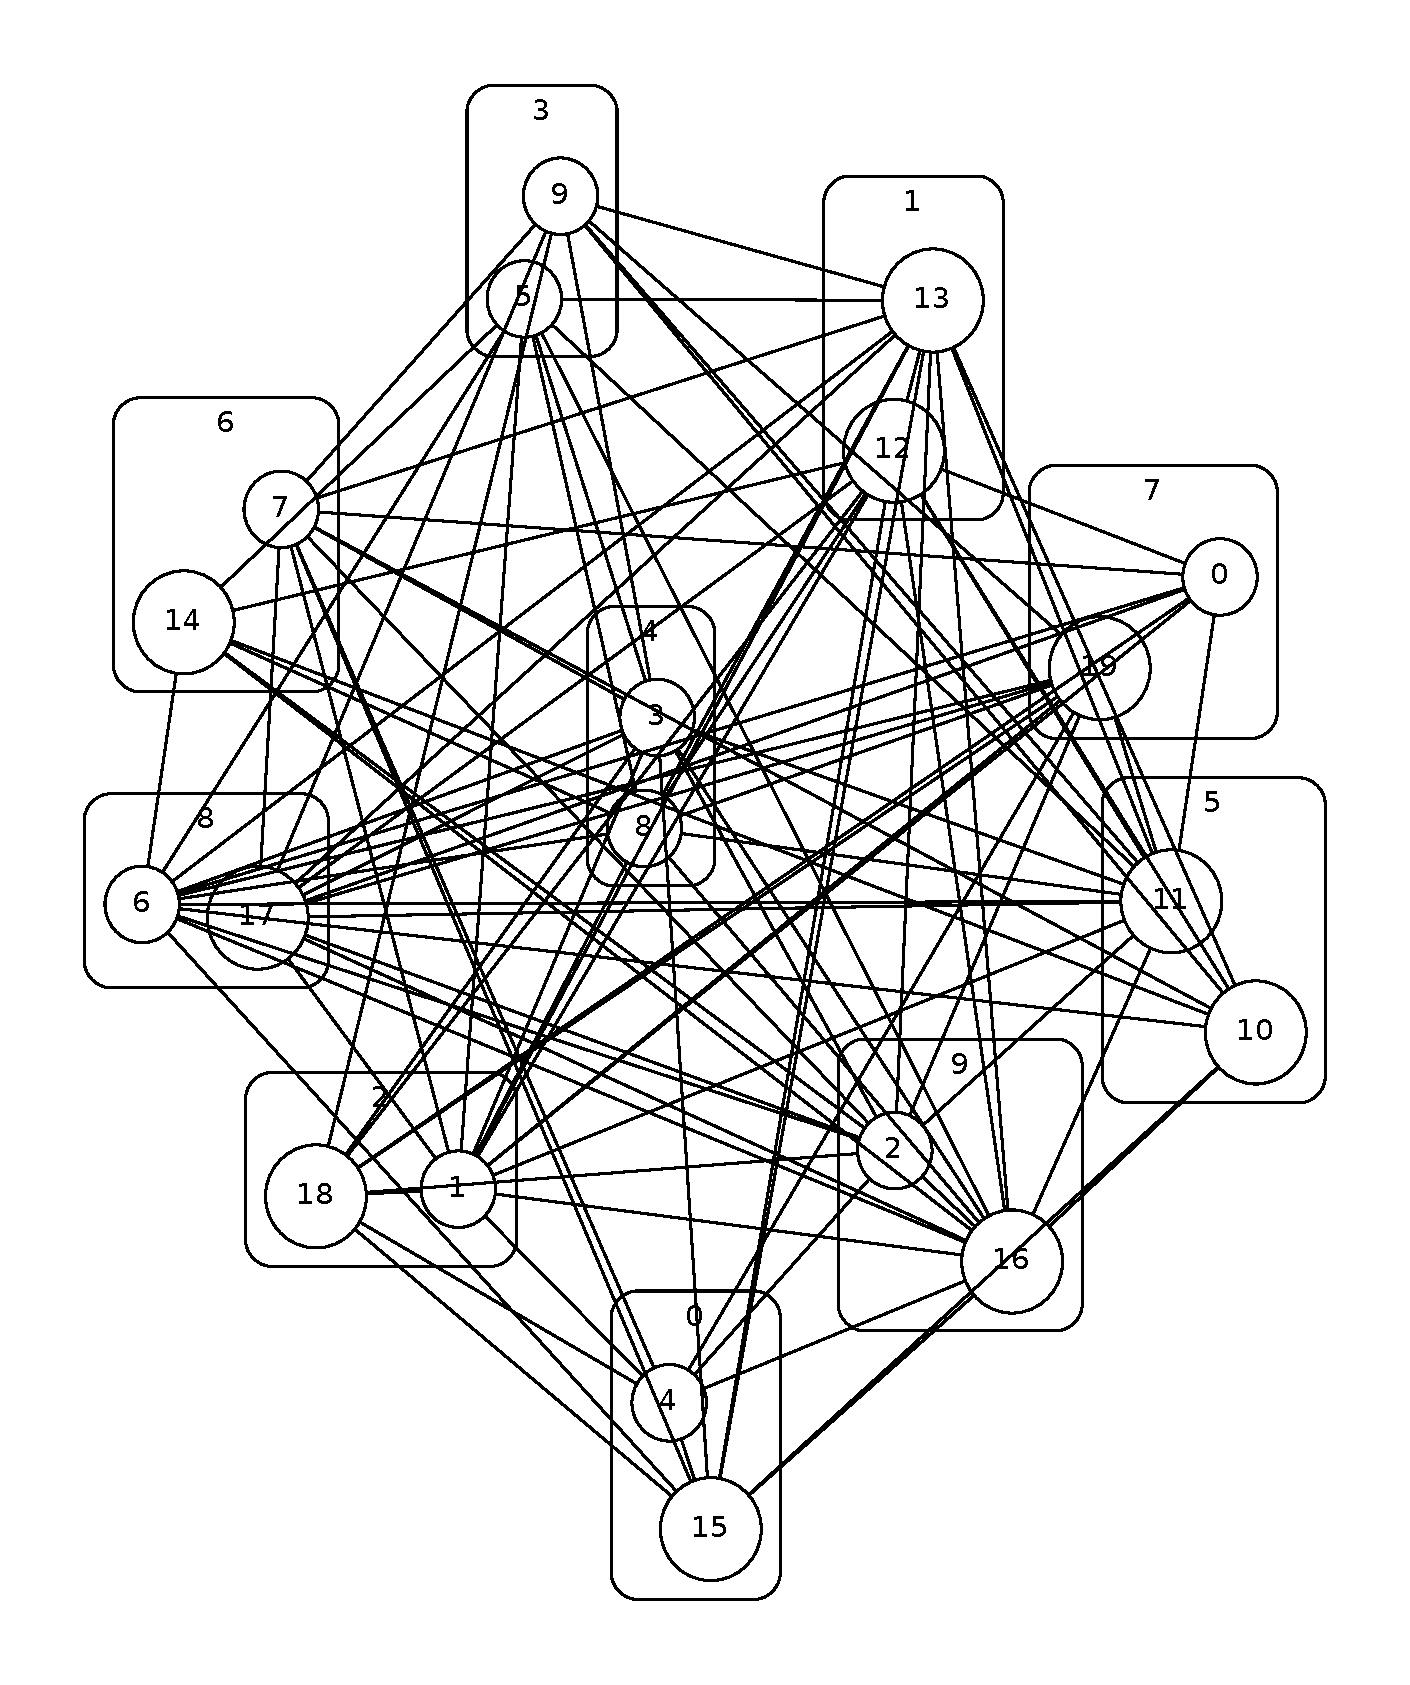
\includegraphics[width=\textwidth]{../img/graphviz-post}
		\caption{Konfliktgraph der Instanz selbst}
		\label{fig:graphviz:pre}
	\end{subfigure}
	\begin{subfigure}[t]{0.45\textwidth}
		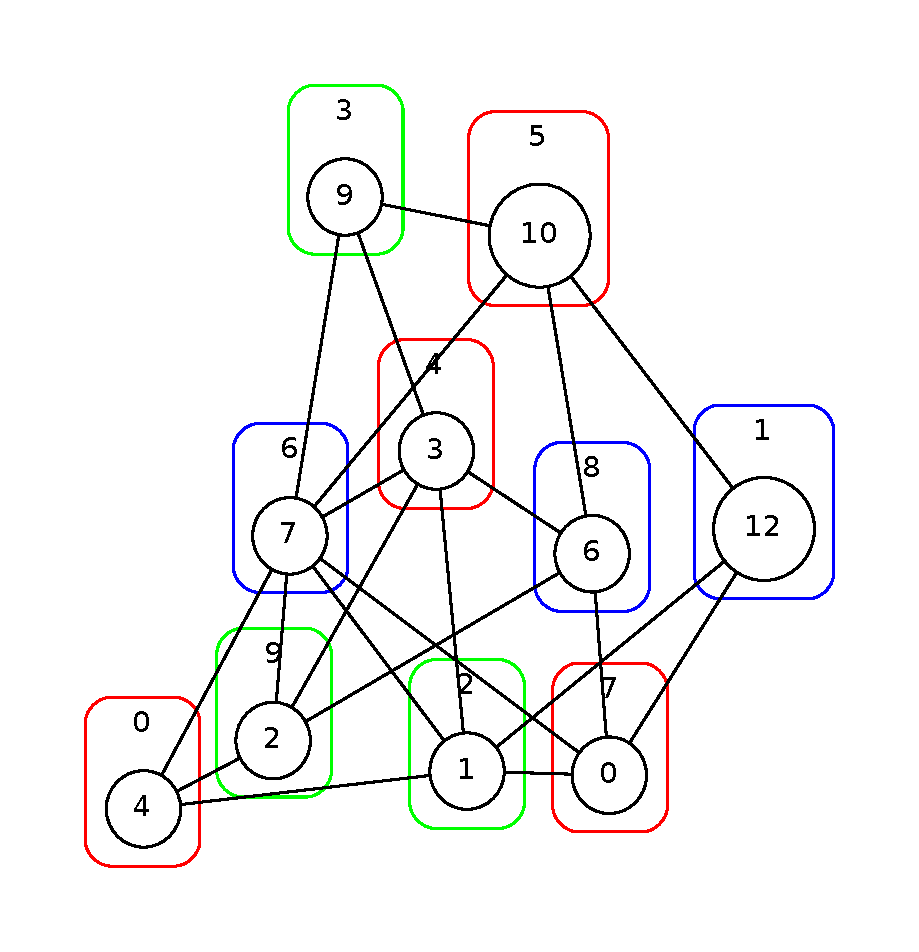
\includegraphics[width=\textwidth]{../img/graphviz-pre}
		\caption{Eine mögliche Lösung (eingefärbter und vereinfachter Konfliktgraph)}
		\label{fig:graphviz:post}
	\end{subfigure}
	\label{fig:graphviz}
	\caption{Beispiel der Darstellung von Probleminstanzen und -lösungen durch Graphviz, anhand von \texttt{Table2\_random\_instances/n20p5t2s5.pcp}.}
\end{figure}

Eingeschränkt wurde der Einsatz von Graphviz durch die Tatsache, dass bei großen Pro\-blem\-in\-stan\-zen natürlich auch die Lösungsgröße entsprechend anwächst und daher ein hän\-disch\-er Vergleich nur noch schwer bis gar nicht möglich
ist. Daher wurde Graphviz vor allem dazu eingesetzt, die Selbsttestung des Programmes zu überprüfen und mehrere Szenarien zu kreieren, welche zu Problemen im Programmablauf führen könnten. Mit diesen Szenarien
kon\-nte dann verifiziert werden, dass das Programm in der Lage ist, ungültige Lösungen von selbst auszuschließen.


\section{Ubigraph}
\label{sec:ubigraph}
Bei \textit{Ubigraph}\footnote{\url{http://ubietylab.net/ubigraph/}} handelt es sich um eine Plattform zur visuellen Darstellung von Graphen. Die Plattform besteht einerseits aus einem Server, welcher Befehle entgegen nimmt und aus diesen Befehlen eine 
dreidimensionale Darstellung des Graphen ausgibt und andererseits aus einer Vielzahl an Schnittstellen für alle nur erdenklichen Programmiersprachen. Mit Hilfe von Ubigraph ist es möglich, die
Vorgänge innerhalb der VNS, sowie beim Aufbau der Initiallösung zeitnah mitzuverfolgen und gleichzeitig eine ansehnliche dreidimensionale Darstellung des Graphen zu erlangen.

\begin{figure}
\centering
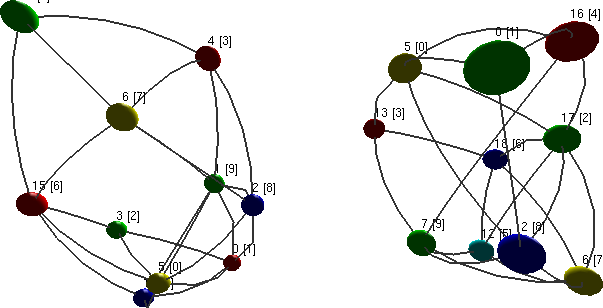
\includegraphics[width=0.5\textwidth]{img/ubigraph.png}
\caption[Ein Beispiel der graphischen Ausgabe der Ubigraph-Software]{Ein Beispiel der graphischen Ausgabe der Ubigraph-Software. Zu sehen ist die Ausgabe der finalen Lösung der VNS, welche bereits mehrere Nachbarschaften durchlaufen hat.}
\label{img:ubigraph}
\end{figure}
Bei der Serversoftware handelt es sich um ein Stück proprietären Code, welcher per XML-RPCs angesprochen werden kann. Der Server nutzt OpenGL, um die gezeichneten Graphen per Grafikkarte darzustellen. Als
Schnittstelle dienen \textit{Remote Procedure Calls (RPC)}, welche per \textit{Hyper Text Transfer Protocol (HTTP)} an den Server übermittelt werden. Der Name XML-RPC stammt von der Auszeichnungssprache
\textit{Extensible Markup Languag (XML)}, was soviel heißt wie Erweiterbare Auszeichnungssprache, welche als Anfrage- und Antwortsprache verwendet wird. Die Daten einer solchen Anfrage werden von der
ausgeführten Software per HTTP-POST-Methode an den Server übermittelt, welcher auch wieder eine XML-Meldung über Erfolg oder Misserfolg der Operation zurückliefert. 

Da es sich bei XML-RPC um einen textbasierten Standard handelt, ist vor allem die Integration von Ubigraph in Skriptsprachen besonders einfach. Für viele Sprachen werden bereits Schnittstellen mitgeliefert,
welche eine noch einfachere Verwendung von Ubigraph ermöglichen. Der Quellcode dieser Schnittstellen ist als Open-Source-Software zur Verfügung gestellt und kann daher ebenso eingesehen werden wie die
Spezifikation für die Server-Schnittstelle per RPC\@. Da für C++ selbst keine eigene Schnittstelle vorhanden war, wurde auf die Schnittstelle für C zurückgegriffen, welche sich wiederum einiger anderen Bibliotheken
aus dem XML und RPC-Umfeld bedient. Da C++ die Möglichkeit bietet, nahtlos mit C-Code umzugehen, war die Integration von Ubigraph keine große Herausforderung. Die Ubigraphschnittstelle für C bietet einige
einfache Optionen zum Zeichnen von Knoten, Kanten beziehungsweise der Manipulation der Eigenschaften derselben, wie z.~B.\ Farbe, Form und Beschriftung.
